% phone type
% alignment
% 寫資料集
% 最後!處理數據作圖…!! 是要多久……啊就那樣

\chapter{單一語音離散表徵與音位的關係}  % 與語音標記的對應模式
  
由於 HuBERT 和 wav2vec 2.0 等語音基石模型的成功,不但在語音任務上達到了前所未有的表現,還促使從語音表徵離散化的想法得以發展。以此產生的「無文字(Textless)」架構,讓人們在處理語音訊號時,有了連續表徵以外的新選擇。
離散形式的表徵,可以直接應用文字領域發展的技術,如機器翻譯、生成式模型等,為語音技術帶來新的突破。
另一方面,基於離散「符記(token)」的共同形式,離散語音表徵可以更好的整合文字資料,促成多模態領域的發展。跨模態離散表徵的成功,甚至驅使影像領域也開始嘗試發展離散表徵,如探討唇語的 AV-HuBERT \cite{shi2021learning} 等等,展現了離散表徵在資料處理上的優勢。  % 不是模型運算
% 還有影像的 vokenization \cite{tan-bansal-2020-vokenization} 等等。好像更早
% TODO: 找到影像那邊的新的 token?

% 語言學那邊只有一般語音?還是包含 acoustic phon 嗎?
此外,除了技術的角度切入,為了探討離散語音表徵成功背後的可能因素,
以及它們和語言學對人類語音理解之間的差異,甚至是進而得以利用這些技術協助他們更細緻的探討人類的語音現象。因此,原先在連續語音表徵上的語音學分析,也開始關注離散表徵背後有多能描述對語音現象,將其列入考量,成為除了連續語音特徵和時頻譜之外的另一個選擇。
% TODO: cite  "is cont necessary? 那篇"
% 更由於這些離散表徵形式上和音位、文字的相似性,  %% 這個好像還沒?
%% 他們還是更喜歡 IPA,只是先當成一種新的 label 吧?

\section{相關研究}

\subsection{無文字與離散語音表徵}
  
自從 HuBERT 帶起來的研究之後,愈來愈多離散表徵相關的研究,例如 \mycite{這邊要 cite 一些東西} 等等。它們在提出自己的離散表徵時,也會採用原先 HuBERT 提供的那些衡量方式,
% 例如 PNMI 等等的,
來驗證這些離散單元確實是與語音中的內容與人類對語音的詮釋具有一定程度的相關性,並從消息理論的角度,證明這些偽標記找出來的符號之間,確實可以做到區分語音中不同形式的資訊。

\subsection{語音學分析}
  
另一個層面,由於語音處理本身所針對與探討的終究是人類的語音。因此,有一群研究者通過對人類語音本身的理解,將這些知識應用在分析模型如何對語音訊號建構表徵之上。例如  \mycite{這邊要 cite 那些如唐顥等分析語音本身的} 等。
% 就韋誠說的妹子那篇嗎?

基於這些作品都對語音的離散表徵感到興趣而做出的探討,本論文也先透過過往幾個常用來分析語音表徵的方式,特別是HuBERT 原始 paper 中提出的標準進行初步的分析。以下介紹此次分析語音表徵的衡量方式:

\section{衡量方式}

  
首先是純度(Purity)、熵(Entropy)和相互資訊(Mutual Information,MI),
這類標準是在原始 HuBERT 論文中採用的指標 \cite{hsu_hubert_2021, hsu_hubert_2021-2},
在比對機器學習過程得到的偽標記與人類知識的標註之間,兩者的相關性(Correlation)。
以下對各標準進行詳細解釋:


不論是什麼語音基石模型,語音表徵的基本單位是音框(Frame)。因此一段語句(Utterance)的語音的離散單元被表示為 $[y_1, \cdots\cdots, y_T]$。其中 $T$ 是該段語句的音框總數。對於該段語句,若給予一段在音框上對齊的語音學標註(Phonetic Label)
$[z_1, \cdots\cdots, z_T]$,此時我們可以將離散單元與標註之間配對的出現次數,寫為一個雙變數的共同分佈(Joint Distribution)

$$
p_{yz} = 
\frac{
\sum^T_{t=1}
[
{y_t = i 
\wedge
z_t = j}
]
}
{T}$$

其中 $i$ 是第 $i$ 個音位類別,而 $j$ 指編號為$j$的離散單元。
兩個變數的邊際機率(Marginal Probability)為
$$p_z(j)=\sum_i{p_{yz}(i, j)}$$
和
$$p_y(i)=\sum_j{p_{yz}(i, j)}$$

因此,對於每一個音位 $i$ 而言,這個音位對應最可能的離散單元為
 $$z^\ast(i) = \arg\max_j p_{yz}(i, j)$$
與之相對應的,對於每一個離散單元的類別 $j$ 則可以找到機率最高的音位
$$y^\ast(j) = \arg\max_i p_{yz}(i,j)$$

於是我們可以計算出以下指標:

\subsection{純度}

本指標考慮音位和離散單元兩個序列之間對應的最高機率,因此從音位與離散單元的角度出發,可以得到以下兩項數據:


%% 這邊抄 HUBERT paper
\paragraph{音位純度(Phoneme Purity)}
考慮每個離散單元對應的音位中,最高機率音位的機率,表示為

% phoneme purity: 每個cluster unit內的phoneme purity,代表此unit是否有phoneme代表性

% Expectation symbol
\newcommand{\E}{\mathbb{E}}

$$\E_{p_z(j)}\left[p_{y|z}(y^*(j)|j) \right]$$

此指標表示該單元是否對與它對應的音位有足夠的代表性。

\paragraph{分群純度(Cluster Purity)}
與音位純度相對,改以每個音位的角度,考慮對應單元類別的機率

$$\E_{p_y(i)}\left[p_{z|y}(z^*(i)|i) \right]$$

由於離散表徵進行分群演算法時的類別數是一項超參數(Hyperparameter),且通常離散單元的分群數量會比音位多,因此該統計數據本身不直接具有語音學的解釋意義,而且在分群數量很多時會顯著下降。

然而該指標在考量音位純度時必須一併考慮,因為當分群數非常多時,分群純度過低可能使得音位純度相較失去意義。一個極端的情形是每一個音框都給予不同的離散單元編號,如此音位純度可以達到 100\%。但如此一來,離散單元做不到歸納音位類別的目的,音位純度也就失去了意義。



% cluster purity:每個phoneme對應到的cluster統計,若cluster purity低代表less liguistical meaning?單一 phoneme 本身對應的 unit 的一致性。如果


\subsection{熵和相互資訊}
  
除了純度提供「最高機率」的對應關係,根據 HuBERT 論文 \cite{hsu_hubert_2021-2} 中的分析方式,我們也可以從資訊理論(Information Theory)的角度,觀察兩個序列的熵和相互資訊。

\paragraph{熵}

熵的定義按照資訊理論,衡量兩個序列中標籤類別出現機率的不確定性(Uncertainty),公式寫作:

\begin{align}
    H(y) = \sum_i{p_y(i)\log p_y(i)}
    H(z) = \sum_j{p_z(j)\log p_z(j)}
\end{align}

$H(y)$ 和 $H(z)$ 分別為音位和離散單元的熵。

\paragraph{以音位標準化之相互資訊(Phone-normalized Mutual Information,PNMI)}

本數據以「觀察到某一個離散單元,能降低多少音位標註的不確定性」,定義該離散單元的出現背後提供了多少音位的資訊。公式寫為:
\begin{align}
\frac{I(y;z)}{H(y)}&=\cfrac{\sum_i \sum_j p_{yz}(i, j) \log \cfrac{p_{yz}(i, j)}{p_y(i)p_z(j)}}{\sum_i p_y(i) \log p_y(i)} \\
&=\frac{H(y)-H(y|z)}{H(y)} \\
&=1-\frac{H(y|z)}{H(y)}
\end{align}

該項數據愈高,表示離散單元的分群愈是足以提供語音音位的資訊,是一個品質更好的分群結果。
由於離散單元能多好的對應到音位才是人們所關心的問題,因此與純度不同,只以音位的角度出發,而不考慮以離散單元分群的角度。



\section{實驗集與分析模型}
  
本研究的分析對象參考無文字架構 \cite{noauthor_textless_2021, lakhotia_generative_2021, lakhotia_generative_2021-1}  研究,採用當中提及的 CPC、Wav2vec 2.0 和 HuBERT 三個語音基石模型,並與作為比對的聲學特徵梅爾時頻譜(Mel-Spectrogram),一共四種語音表徵模型。
$$
\text{((寫一下 resolution 跟層數))}
$$
此後亦跟隨該研究選用特定模型層數,和其釋出的K-平均量化模型。
%% ==========
這些模型層數與量化為該研究中被證明與語音學特徵最相關,且被使用於無文字架構後續研究之語音離散表徵的抽取方法。
%% ==========
無文字研究中已透過 (某某) 語料對四種語音表徵進行 K-平均分群演算法,分別得到群數為 50、100 和 200 的三個量化模型。

%% ==========
本論文以公開的 LibriSpeech 資料集為分析對象,採取其 train-clean-100 為分析的語音語料庫。
%% ==========
% 因此,
本研究將語音語料庫的語音資料經過四個模型獲取連續表徵後,再經過量化模型得到完全由離散單元組成的「偽文字」語料。

%% ==========
針對語音學的音位標註,吾人透過 Montreal 強迫對齊器(Forced-Aligner) [[CITE montreal]] 的英語預訓練模型, 從語料庫的文字轉寫 取得 語音資料的音位標註 與對應的時間範圍。 最後透過 語音表徵各自的 時間解析度 生成 以音框為單位的 音位標註語料。
最後將兩者對語音資料集進行音位標註相關性的分析。



\section{分析結果}



%% \begin{center}
%% (((還是放一下長條圖說個事兒好了)))     
%% \end{center}
  
由表 \ref{tab:grouped_tables} 中可以看出,分群的群數愈多時,音位的純度確實有所上升,但這可能是犧牲分群純度得來的。因此再看 PNMI 的指標可以發現,整體離散單元和音位標註的相關性還是有所提升的。

此外,就不同模型來觀察,HuBERT 的表現是四種語音表徵之中最好的,一定程度上可以佐證 HuBERT 在找出語音中有意義單位上的效能,以及為什麼無文字架構通常以 HuBERT 當成抽取語音離散表徵的模型。



% \begin{figure}
%     \centering
%     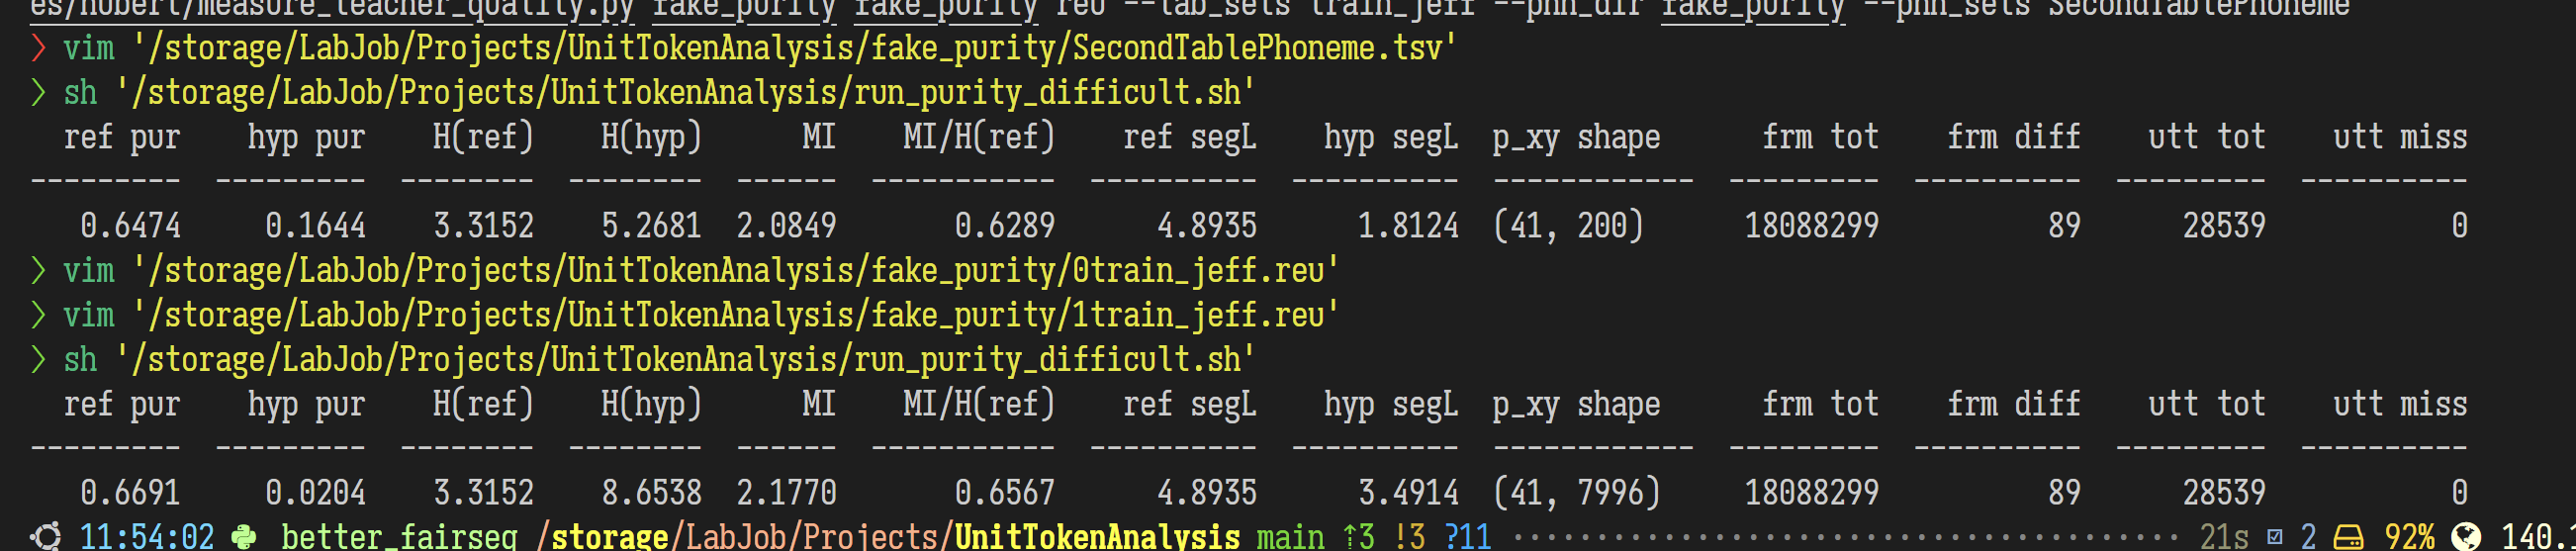
\includegraphics[width=0.75\linewidth]{figures/res1.png}
%     \caption{Enter Caption}
%     \label{fig:enter-label}
% \end{figure}








%% \documentclass{article}
%% \usepackage{caption}
%% \usepackage{subcaption}


\begin{table}[!htbp]
    \centering
    \begin{subtable}[t]{\textwidth}
        \centering
        \begin{tabular}{cccccc}
            %% 0 & refpur & hyppur & Href & Hhyp & MI\_pnmi\\
            & 音位純度 & 分群純度 & 音位熵 & 離散單元熵 & PNMI \\
            HuBERT      &   0.5256   &  0.3382 &   3.3152  &  3.8681    &     0.4993   \\   %% 1.6552 h
            wav2vec 2.0 &   0.4006   &  0.2676 &   3.3152  &  3.8215    &     0.3706   \\   %% 1.2286 w
            CPC         &   0.5188   &  0.3812 &   3.3146  &  3.7918    &     0.4992   \\   %% 1.6545 c
            LogMel      &   0.3253   &  0.1473 &   3.3158  &  3.8630    &     0.2647   \\   %% 0.8776 l
        \end{tabular}
        \caption{群數 = 50}
        \label{tab:ch3-clu050}
    \end{subtable}

    \vspace{0.5cm}

    \begin{subtable}[t]{\textwidth}
        \centering
        \begin{tabular}{cccccc}
            %% 0 & refpur & hyppur & Href & Hhyp & MI\_pnmi\\
            & 音位純度 & 分群純度 & 音位熵 & 離散單元熵 & PNMI \\
            HuBERT      &   0.6097   &  0.2553 &   3.3152  &  4.5704    &     0.5786   \\   %% 1.9181 h
            wav2vec 2.0 &   0.4877   &  0.2118 &   3.3152  &  4.5284    &     0.4596   \\   %% 1.5235 w
            CPC         &   0.5895   &  0.2674 &   3.3146  &  4.5034    &     0.5557   \\   %% 1.8418 c
            LogMel      &   0.3348   &  0.0931 &   3.3158  &  4.5591    &     0.2789   \\   %% 0.9247 l
        \end{tabular}
        \caption{群數 = 100}
        \label{tab:ch3-clu100}
    \end{subtable}

    \vspace{0.5cm}

    \begin{subtable}[t]{\textwidth}
        \centering
        \begin{tabular}{cccccc}
            %% 0 & refpur & hyppur & Href & Hhyp & MI\_pnmi\\
            & 音位純度 & 分群純度 & 音位熵 & 離散單元熵 & PNMI \\
            HuBERT      &   0.6474   &  0.1644 &   3.3152  &  5.2681    &     0.6289   \\   %% 2.0849 h
            wav2vec 2.0 &   0.5427   &  0.1467 &   3.3152  &  5.2173    &     0.5188   \\   %% 1.7199 w
            CPC         &   0.6098   &  0.1789 &   3.3146  &  5.1885    &     0.5882   \\   %% 1.9497 c
            LogMel      &   0.3474   &  0.0569 &   3.3158  &  5.2322    &     0.2955   \\   %% 0.9798 l
        \end{tabular}
        \caption{群數 = 200}
        \label{tab:ch3-clu200}
    \end{subtable}

    \caption{Grouped Tables}
    \label{tab:grouped_tables}
\end{table}





 

\section{本章總結}

  
本章節探討以音框為單位取出的語音離散表徵
與對應的音位標註之間的關係,
從分析結果中可以得到,
HuBERT 模型
的離散表徵
確實
與
人類
理解的
語音單位
「音位」
之間,
具有最明顯的相似性,
也進一步證明
% 以此尋找語音中的
為何
HuBERT 目前是
抽取語音離散表徵時最常使用的模型。


% 第二塊 %%%%%%%%%%%%%%%%%%

% 第一塊 %%%%%%%%%%%%%%%%%%
%%%%%% \subsection{基於各自音位的分析}

%%%%%%%%% (放數據)



% 第一塊後半 %%%%%%%%%%%%%%%%%%









% 後面寫 arpabet?

% 調音部位 →    唇   舌冠  舌背  咽喉
% 調音方法 ↓    雙唇  唇齒  舌唇  齒   齒齦  齦後  捲舌  齦腭  硬腭  軟腭  小舌  咽   會⁠厭 聲門
% 鼻音    m̥  m       ɱ       n̼          n̥  n           ɳ̊  ɳ           ɲ̊  ɲ   ŋ̊  ŋ       ɴ                       
% 塞音    p   b   p̪  b̪  t̼  d̼          t   d           ʈ   ɖ           c   ɟ   k   ɡ   q   ɢ           ʡ       ʔ   
% 有噝擦音                                  s   z   ʃ   ʒ   ʂ   ʐ   ɕ   ʑ                                               
% 無噝擦音  ɸ   β   f   v   θ̼  ð̼  θ   ð   θ̠  ð̠  ɹ̠̊˔    ɹ̠˔     ɻ˔          ç   ʝ   x   ɣ   χ   ʁ   ħ   ʕ   ʜ   ʢ   h   ɦ
% 近音            ʋ̥  ʋ                   ɹ̥  ɹ           ɻ̊  ɻ           j̊  j   ɰ̊  ɰ                               ʔ̞
% 閃音        ⱱ̟      ⱱ       ɾ̼          ɾ̥  ɾ           ɽ̊  ɽ                               ɢ̆              ʡ̆      
% 顫音    ʙ̥  ʙ                           r̥  r           ɽ̊r̥    ɽr                          ʀ̥  ʀ                       
% 邊擦音                                   ɬ   ɮ           ɭ̊˔ ɭ˔          ʎ̝̊ ʎ̝  ʟ̝̊ ʟ̝                              
% 邊近音                                   l̥  l           ɭ̊  ɭ           ʎ̥  ʎ   ʟ̥  ʟ       ʟ̠                      
% 邊閃音                                       ɺ               ɭ̆              ʎ̆      ʟ̆                              
% 國際音標說明國際音標表模板







%%%% BETTER Have Todo!有機率看哪裡說一下 HuBERT……
%%%% BETTER Have Todo!有機率看哪裡說一下 HuBERT……
%%%% BETTER Have Todo!有機率看哪裡說一下 HuBERT……



%%%%%% \section{語音學分類(phone type)}
%%%%%% 
%%%%%% \subsection{簡介}
%%%%%% 
%%%%%% 除了單一 phn 本身的特性以外,由於 phn 本身彼此不是完全獨立的,而是彼此之間就存在相似的特徵,可以分成幾個組別。因此,依照 CITEME (tanghao等三篇) 的分組方式,對英語的 phn 進行分類並合併比對數據,看看這些 unit 本身是否有 capture 到相似的發聲特徵,而不單純只是把 phn 分成約五十類完全獨立的標籤。
%%%%%% 
%%%%%% % (基於語音表徵本身就是 acoustic sisgnals 來的,應該 by nature 要可以對語音特徵分組吧?)
%%%%%% 
%%%%%% % 以下為各分組進行簡單介紹:
%%%%%% 
%%%%%% % \subsubsection{consonants}
%%%%%% 
%%%%%% 按照發音的方式,子音可分為五類:
%%%%%% 
%%%%%% \begin{itemize}
%%%%%%     \item (Plosive)
%%%%%%     \item 擦音(Fricative)
%%%%%%     \item 塞擦音(Affircate)
%%%%%%     \item 鼻音(Nasal)
%%%%%%     \item 近音(Approximant)
%%%%%% \end{itemize}
%%%%%% 
%%%%%% % \subsubsection{vowels}
%%%%%% 
%%%%%% 母音則是被分為:
%%%%%% 
%%%%%% \begin{itemize}
%%%%%%     \item 單原因
%%%%%%     \item 雙原因
%%%%%% \end{itemize}
%%%%%% 
%%%%%% % 母音在這邊為了簡單起見,會被分在一起?
%%%%%% 
%%%%%% \subsection{解釋意義}
%%%%%% 
%%%%%% \begin{itemize}
%%%%%%     \item 純度(purity):換成type之後有何變化(關聯性更強?)
%%%%%%     \item 熵(entropy)(放直方圖解釋) --> phone type更明顯?
%%%%%%     \item 對齊(alignment):是否減少segment資訊的保留(連續子音母音被合併?
%%%%%% \end{itemize}



%%%%%% 
%%%%%% \subsection{基於語音學分類的分析}
%%%%%% 
%%%%%% (放數據)

%%%%%%%%%%%%%%%%%% \subsection{以語音分段指標衡量對齊(Alignment)程度}
%%%%%%%%%%%%%%%%%%   
%%%%%%%%%%%%%%%%%% 為了分析離散單元跟音位在語句序列之間的對齊程度,
%%%%%%%%%%%%%%%%%% 本研究根據 \cite{strgar_phoneme_2023} 的方法
%%%%%%%%%%%%%%%%%% 採用語音分段(Speech Segmentation)的標準去衡量。
%%%%%%%%%%%%%%%%%% 具體動機為將被分到同一個離散單元編號的音框當成語音分段的同一類別的音位,
%%%%%%%%%%%%%%%%%% 以此
%%%%%%%%%%%%%%%%%% 期望可以
%%%%%%%%%%%%%%%%%% 觀察出
%%%%%%%%%%%%%%%%%% 在每一段語句中,
%%%%%%%%%%%%%%%%%% 離散單元出現的順序與範圍,
%%%%%%%%%%%%%%%%%% 與音位標註指示的範圍一致的程度。
%%%%%%%%%%%%%%%%%% 
%%%%%%%%%%%%%%%%%% %% alignment

% 看 alignment 並 cite 那邊,說明一下
% 寫子母音

%%%%%%%%% 糟糕,沒講 HuBERT 但隨便
